\documentclass[]{article}

\usepackage{mypreamble}

\usepackage[nonumberlist,nogroupskip]{glossaries}

\setglossarystyle{super}

\newglossaryentry{ipm}{
    name={Incremental PM},
    description={Incremental Personal Model}
}

\newglossaryentry{gpm}{
    name={Warm start PM},
    description={Warm start Personal Model}
}

\newglossaryentry{pm}{
    name={PM},
    description={Personal Model}
}
\newglossaryentry{ib}
{
name={iButton},
description={Wireless temperature sensors},
plural={iButtons},
firstplural={iButtons}
}

\newglossaryentry{ubibot}
{
name={UbiBot},
description={Wireless environmental sensor},
}

\newglossaryentry{7730}
{
name={ISO~7730:2005},
description={ISO~7730:2005 is a thermal comfort standard developed by ISO}
}

\newglossaryentry{55}
{
name={ASHRAE~55--2020},
description={ASHRAE~55--2020 is a thermal comfort standard developed by ANSI and ASHRAE}
}

\newglossaryentry{lr}{
name={Logistic Regression},
description={Logistic Regression model}
}

\newglossaryentry{mlp}{
name={Multi-Layer Perceptron},
description={Multi-Layer Perceptron model}
}

\newglossaryentry{rdf}{
name={Random Forest},
description={Random Forest model}
}


\newglossaryentry{shap}{
name={SHAP},
description={SHapley Additive exPlanations}
}

%\makenoidxglossaries

\usepackage{geometry}
\geometry{
    a4paper,
    margin=25mm,
}

\begin{document}

\section{Appendix}

    \section*{Nomenclature}
\renewcommand{\baselinestretch}{0.75}\normalsize
\renewcommand{\aclabelfont}[1]{\textsc{\acsfont{#1}}}
\begin{acronym}[longest]

    \acro{hr}[$\mathit{HR}$]{heart rate\acroextra{, beats per minute}}
    \acro{pmv}[PMV]{Predicted Mean Vote}
    \acro{rhrn}[RHRN]{Right-Here-Right-Now}
    \acro{svm}[SVM]{Support Vector Machine}
    \acro{t-db}[$t_{i}$]{indoor air temperature\acroextra{, $^{\circ}$C}}
    \acro{t-nb}[$t_{nb,w}$]{wrist near body temperature\acroextra{, $^{\circ}$C}}
    \acro{t-sk}[$t_{sk}$]{skin temperature\acroextra{, $^{\circ}$C}}
    \acro{t-sk-w}[$t_{sk,w}$]{wrist skin temperature\acroextra{, $^{\circ}$C}}
    \acro{w-i}[$W_{i}$]{humidity ratio indoors\acroextra{, kg$_{water\:vapor}$/kg$_{dry\:air}$}}

\end{acronym}
\renewcommand{\baselinestretch}{1}\normalsize

\appendix

\renewcommand\thefigure{\thesection.\arabic{figure}} 
\renewcommand\thetable{\thesection.\arabic{table}} 

\section{Methodology}\label{sec:methodology2}

\subsection{Sensors}\label{subsec:sensors}

We used Fitbit Versa smartwatches since they are capable of accurately continuously tracking \ac{hr}~\cite{Nelson2019} and have a touch screen that can be used to complete \ac{rhrn} surveys using the Cozie clock-face.

\glspl{ib} are wireless temperature sensors that can accurately measure and log \ac{t-sk}~\cite{VanMarkenLichtenbelt2006}.
We selected a 180~s sampling period, hence each \gls{ib} could record data for approximately 127 days.
A sampling period of 180~s provides reasonably accurate results while limiting to two the number of times that data had to be downloaded throughout our study~\cite{Tartarini2020d}.

Participants were asked to install Netatmo Smart Home Weather Station weather stations (NWS03, Netatmo, France) in the room of their house, where they spent the majority of their time indoors.
The indoor module was used to monitor \ac{t-db} and relative humidity.

A \gls{ubibot} WS1 Pro (\gls{ubibot}, China) was used to measure and log \ac{t-db} and relative humidity at the participant's workplace.
Participants installed the \gls{ubibot} on their work desk far away from heat sources.

Each participant also installed an \gls{ib} (model DS1925) on a bag/backpack of their choice.

\begin{table}[h!]
    \centering
    \caption{Sensors specifications.}
    \label{tab:table-accuracy}
    \small
\begin{tabular}{ccccc}
    \toprule
\begin{tabular}[c]{@{}c@{}}Manufacturer -\\Product name\end{tabular}         & Location            & \begin{tabular}[c]{@{}c@{}}Variables\\Measured\end{tabular}                                                          & \begin{tabular}[c]{@{}c@{}}Accuracy\\Manufacturer
\end{tabular} & Range                   \\
    \midrule
    \begin{tabular}[c]{@{}c@{}}Fitbit --\\Versa\end{tabular}     & \begin{tabular}[c]{@{}c@{}}Non-dominant\\wrist\end{tabular}  & \ac{hr}           & \begin{tabular}[c]{@{}c@{}}Not reported\\91~\%~\cite{Nelson2019}\end{tabular}                                               & Not reported            \\
\begin{tabular}[c]{@{}c@{}}Netatmo --\\Smart Home\\Weather Station\end{tabular} & Home                & \begin{tabular}[c]{@{}c@{}}\ac{t-db}\\RH\end{tabular} & \begin{tabular}[c]{@{}c@{}}$\pm 0.3 ^{\circ}$C\\$\pm 3$~\%
\end{tabular}                                                                & \begin{tabular}[c]{@{}c@{}}0 to 50~$^{\circ}$C\\0 to 100~\%
\end{tabular}  \\
\begin{tabular}[c]{@{}c@{}}\gls{ubibot} --\\WS1 Pro\end{tabular}                                                                & Work desk           & \begin{tabular}[c]{@{}c@{}}\ac{t-db}\\RH\end{tabular} & \begin{tabular}[c]{@{}c@{}}$\pm 0.3 ^{\circ}$C\\$\pm 3$~\%
\end{tabular}                                                                  & \begin{tabular}[c]{@{}c@{}}-20 to 60~$^{\circ}$C\\1 to 90~\%
\end{tabular} \\
\begin{tabular}[c]{@{}c@{}}\gls{ib} --\\DS1925\end{tabular}                                                               & Inner wrist         & \ac{t-sk}                                                            & $\pm 0.5 ^{\circ}$C                                                                        & -20 to 85~$^{\circ}$C             \\
\begin{tabular}[c]{@{}c@{}}\gls{ib} --\\DS1925\end{tabular}                                                               & \begin{tabular}[c]{@{}c@{}}Smarwatch\\wristband\end{tabular} & \ac{t-nb}                                                         & $\pm 0.5 ^{\circ}$C                                                                        & -20 to 85~$^{\circ}$C             \\
\begin{tabular}[c]{@{}c@{}}\gls{ib} --\\DS1925\end{tabular}                                                               & Bag                 & \ac{t-db}                                                             & $\pm 0.5 ^{\circ}$C                                                                        & -20 to 85~$^{\circ}$C\\
    \bottomrule
\end{tabular}
\end{table}

\begin{figure}[thb!]
    \centering
    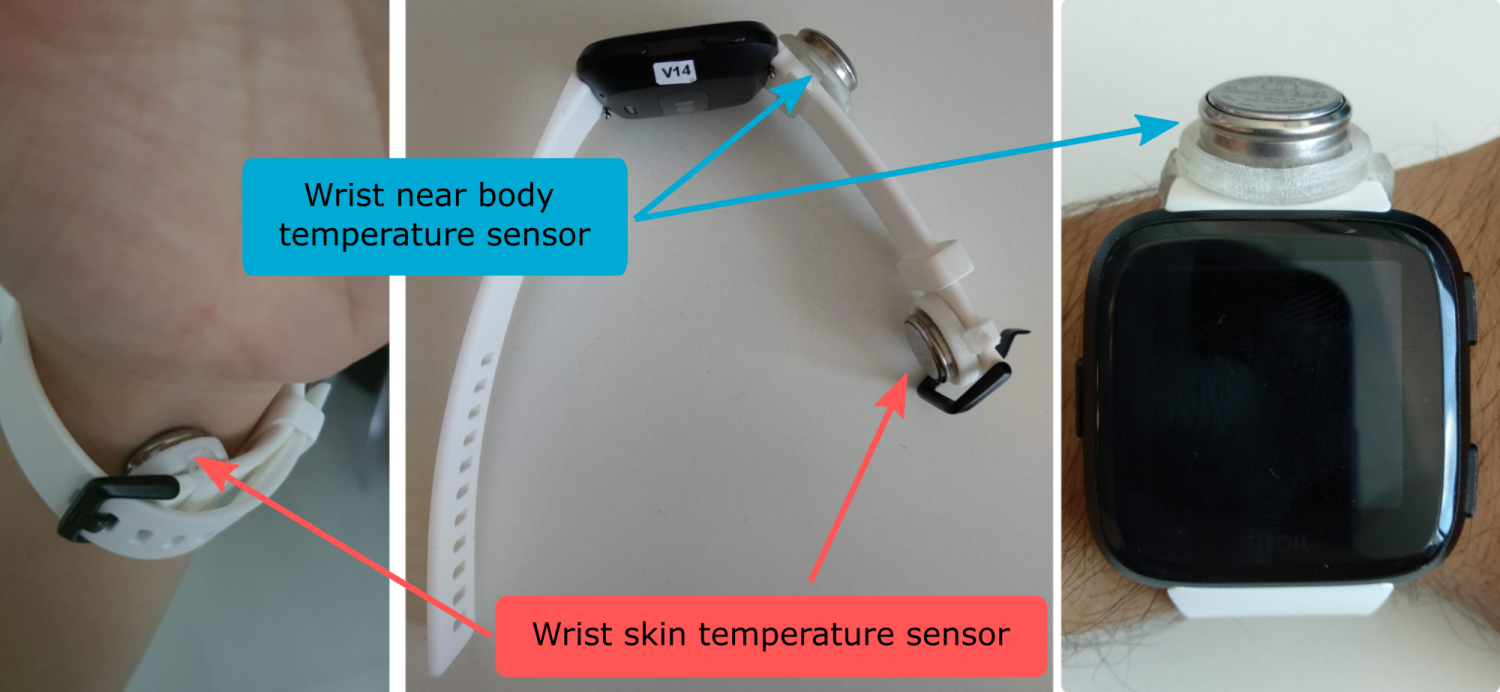
\includegraphics[width=\textwidth]{figures/figure_a1}
    \caption{Fitbit Versa v1 and the two \glspl{ib} we used in this study to measure \ac{t-sk-w} and \ac{t-nb}.}
    \label{fig:ibuttons_fitbit}
\end{figure}

\subsection{Data Analysis}\label{subsec:data-analysis2}

The rationale behind our decision to exclude some of the data collected as stated in Section~2.6.1 is exaplained below.
During exercise, metabolic rate and the body's ability to dissipate heat towards the environment varies extensively among people based on various factors (i.e., weight, age, intensity, and fitness level).
Hence, we excluded surveys completed while the participant was exercising.
Evaluating thermal comfort preference during transitories requires detailed knowledge of all the environmental conditions that occupants were exposed to during and before the event.
Moreover \glspl{ib} may not be suited to measure \ac{t-sk} in these conditions accurately.
Finally, we excluded all the surveys completed when the \ac{t-nb} was at least 1~$^{\circ}$C higher than the \ac{t-sk-w}.
Throughout the data collection period, the outdoor temperature never exceeded 34~$^{\circ}$C consequently, a value of \ac{t-nb} equal or higher than \ac{t-sk-w} can be explained mainly by one of the following conditions: the participant did not wear the smartwatch as recommended, and consequently, the sensor was not in good contact with the skin and its readings were significantly influenced by \ac{t-db} surrounding the occupant;\ the sensor was in contact with another body part, and measured the skin temperature of another body location;\ direct solar radiation heated the sensor.
We also filter out all the surveys completed in less than 3.2~s.
This decision was taken before conducting the field study since we foresaw that some participants may have intentionally tried to take advantage of the study to get the final compensation.
This threshold was the calculated average response speed we obtained by completing 50 surveys as fast as possible.
Entries in the dataset with missing values were dropped from the data analysis.

We analyzed the data using Python v3.8~\cite{pyhton}.
We also used the following Python Packages to perform the analysis: pandas~\cite{reback2020pandas}, scikit-learn~\cite{scikit-learn}, Matplotlib~\cite{Hunter:2007}, seaborn~\cite{waskom2020seaborn}, pythermalcomfort~\cite{Tartarini2020a}, xgboost~\cite{Chen:2016:XST:2939672.2939785}, PsychroLib~\cite{PsychroLib}, numpy~\cite{harris2020array}, and shap~\cite{NIPS2017_7062}.
The lines in the violin plots show the 1st, 2nd (median), and 3rd quartiles.

\begin{table}[htb!]
    \caption{Hyper-parameters used in the grid search.}
    \centering
    \begin{tabular}{cc}
        \toprule
        Model     & Value                                        \\
        \midrule
        \gls{rdf} & \makecell{Number of trees: 100, 300, 500     \\
        Split criterion: Gini index \\
        Min. samples for split: 2, 3, 4 \\
        Min. samples on an edge : 1, 2, 3 \\
        Class weight : balanced
        } \\
        \midrule
        \gls{lr}  & \makecell{Inverse of regularization          \\
        strength: 0.01, 0.1, 1, 10, 100 \\
        Fit intercept: True, False
        } \\
        \midrule
        Extreme Gradient Boosting & \makecell{Number of gradient boosted         \\
        trees: 100, 300, 500 \\
        Maximum tree depth: 2, 4, 6, 8, 10} \\
        \midrule
        \acf{svm} & \makecell{Regularization parameter:          \\
        0.01, 0.1, 1, 10, 100 \\
        Kernel: rbf, sigmoid} \\
        \midrule
        K-Nearest Neighbors  & \makecell{Number of neighbors: 1, 2, 3, 5, 7 \\
        Weights: uniform, distance} \\
        \midrule
        Gaussian Naive Bayes & \makecell{-}                                 \\
        \midrule
        \gls{mlp} & \makecell{Hidden layer size: (13, 13)}       \\
        \bottomrule
    \end{tabular}
    \label{tab:hyperparameters}
\end{table}

\begin{figure}[thbp!]
    \centering
    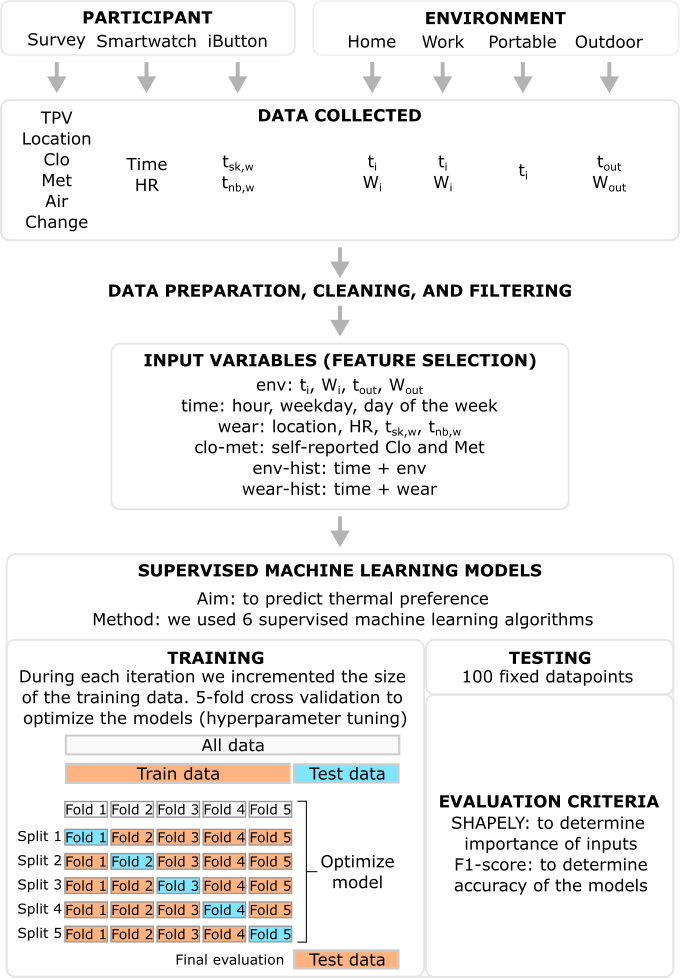
\includegraphics[width=\textwidth]{figures/figure_a2}
    \caption{Flowchart depicting the methodology used used to collect and analyze the data in our study.}
    \label{fig:flowchart}
\end{figure}

\begin{figure}[thbp!]
    \centering
    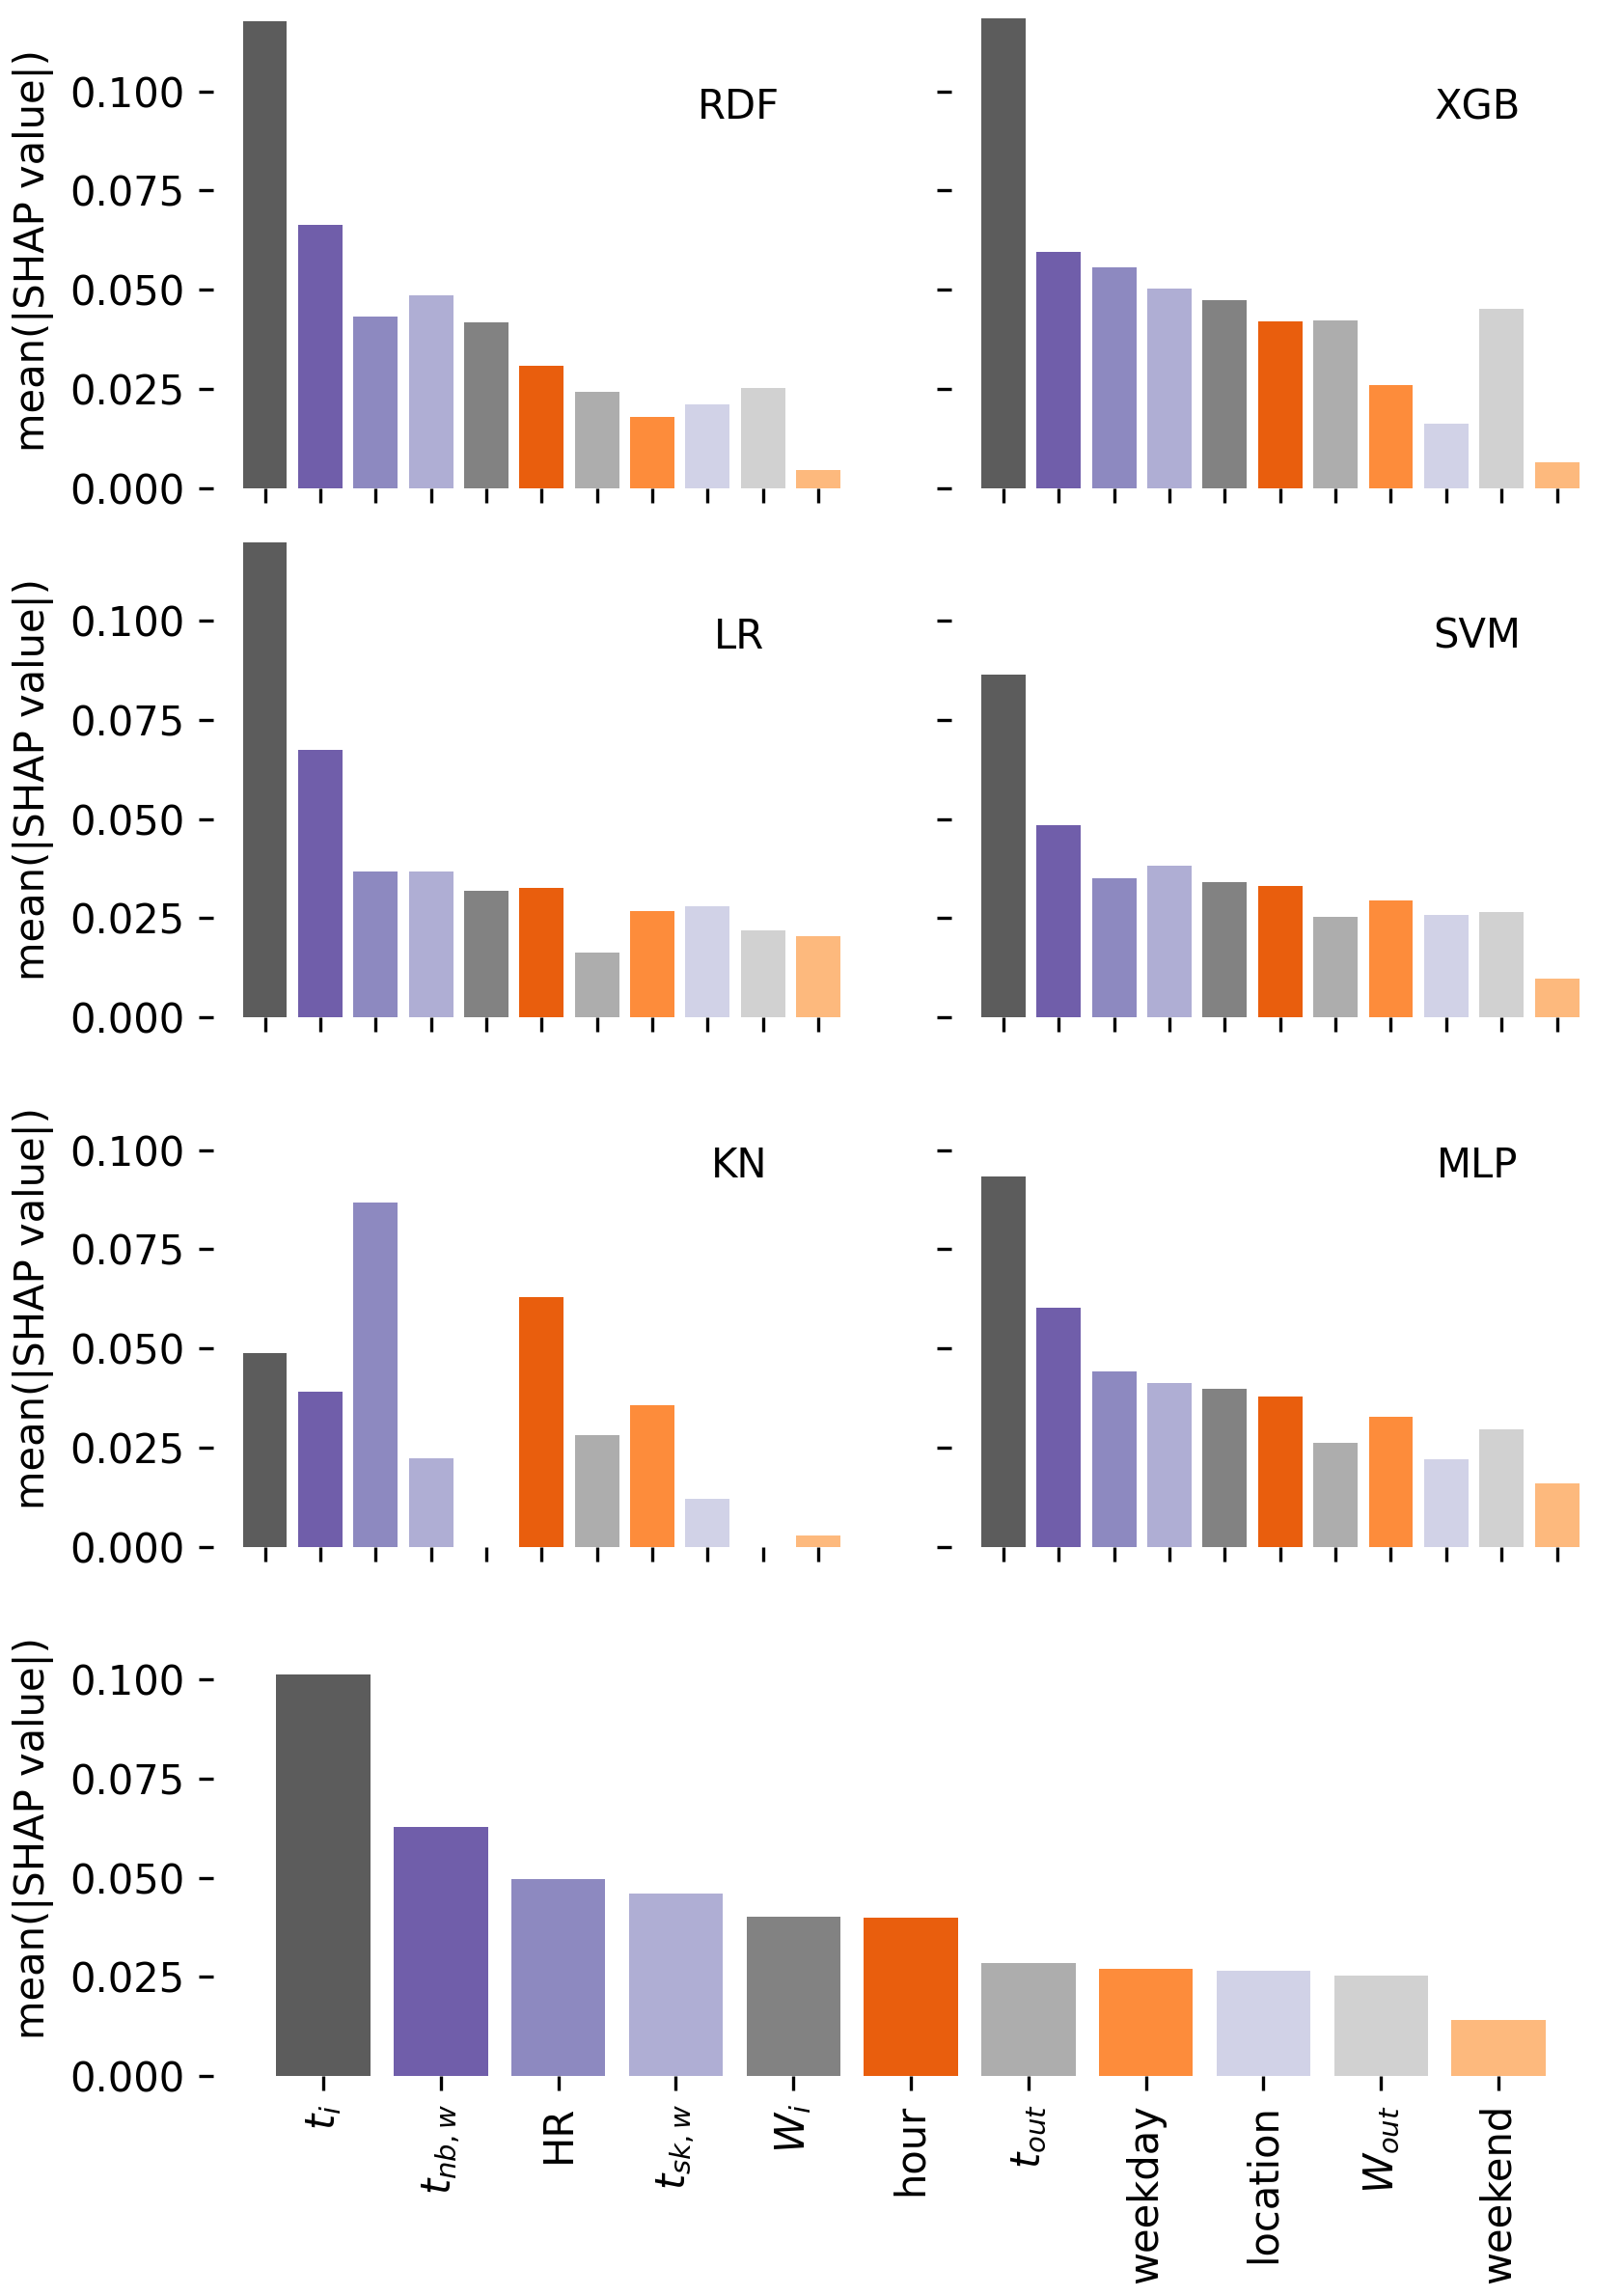
\includegraphics[width=\textwidth]{figures/figure_a3}
    \caption{The \gls{shap} values of the six best performing supervised machine learning models are shown in the top six Figures, while the bottom Figure shows the mean \gls{shap} values of all the six above models.
    Variables are color coded, \emph{environmental} -- using shades of gray, \emph{wearable} -- using shades of purple, and \emph{time} -- using shades of orange.
    Where $t_{out}$ stands for outdoor air temperature, and $W_{out}$ stands for humidity ratio outdoors.}
    \label{fig:shapely_all}
\end{figure}

    \printbibliography

\end{document}